% =====================================================================
% Paper Narrative template (one page, landscape, grayscale)
% Part of the `paper-narrative` skill. Compile with: pdflatex (once).
% Replace the title line and all example content.
% The example content is a neutral toy study (the same one used in the
% argument-tree template); overwrite all of it.
%
% You fill in content, not coordinates:
%   \beat{col}{LABEL}{sentence}          a story beat (gap, idea, payoff)
%   \claim{col}{LABEL}{sentence}         a main claim (1 or 2 per paper)
%   \ev{col}{row}{L|T|N}{solid|partial|missing}{label}{pointer}
%   \stem{col}{number of evidence rows in that column}
%   \verdict{col}{supported|thin|open}{reason}
% =====================================================================
\documentclass[10pt]{article}
\usepackage{mathptmx}\usepackage[scaled=0.9]{helvet}\usepackage[T1]{fontenc}
\usepackage[landscape,margin=0.5in]{geometry}
\usepackage{amsmath,amssymb,enumitem,xcolor}
\usepackage{tikz}
\usetikzlibrary{arrows.meta,shapes.geometric}
\usepackage{microtype}
\renewcommand{\familydefault}{\sfdefault}
\setlist{nosep,leftmargin=1.4em}
\setlength{\parindent}{0pt}
\hyphenpenalty=10000 \exhyphenpenalty=10000 \emergencystretch=2em
\pagestyle{empty}

% ---- Layout. Set \NB to the number of beats and \colw to 25.4/\NB (cm):
%      4 beats: 6.35    5 beats: 5.08    6 beats: 4.23
\newcommand{\NB}{5}
\newcommand{\colw}{5.08}
\newcommand{\beaty}{-1.45}   % centre line of the beat boxes
\newcommand{\evtop}{-3.75}   % first evidence row
\newcommand{\evstep}{1.45}   % distance between evidence rows
\newcommand{\vy}{-9.35}      % verdict strip (room for 4 evidence rows)
\newcommand{\beath}{2.25}    % height of the text area of a beat box
% Six beats make narrow columns; use instead:
%   \beath 3.10   \beaty -1.90   \evtop -4.60   \evstep 1.72   \vy -11.40
% change the bounding box below to {\vy-1.10}, and keep beat sentences to
% about 100 characters and evidence labels to about 40.

\tikzset{
  beatbox/.style={draw=black!70,line width=0.4pt,fill=white,inner sep=5pt,font=\small},
  claimbox/.style={beatbox,draw=black,line width=1.5pt,fill=black!9},
  evbase/.style={inner sep=0pt,font=\scriptsize\bfseries,line width=0.5pt},
  evL/.style={rectangle,minimum size=0.42cm},
  evT/.style={diamond,minimum size=0.60cm},
  evN/.style={circle,minimum size=0.47cm},
  stsolid/.style={fill=black,draw=black,text=white},
  stpartial/.style={fill=white,draw=black},
  stmissing/.style={fill=white,draw=black!55,text=black!55,dash pattern=on 1.5pt off 1.2pt},
  vbase/.style={font=\scriptsize\bfseries,align=center,inner sep=2pt,minimum height=0.5cm,line width=0.5pt,
                text width=\dimexpr\colw cm-0.80cm\relax},
  vsupported/.style={fill=black,draw=black,text=white},
  vthin/.style={fill=white,draw=black},
  vopen/.style={fill=white,draw=black!55,text=black!55,dash pattern=on 1.5pt off 1.2pt},
}
% Fixed-size, top-aligned body so every beat box has the same size and the labels line up.
\newcommand{\beatbody}[2]{\parbox[t][\beath cm][t]{\dimexpr\colw cm-0.95cm\relax}{\raggedright #1\\[3pt]#2}}
\newcommand{\beat}[3]{\node[beatbox] (b#1) at ({(#1-0.5)*\colw},\beaty)
  {\beatbody{{\scriptsize\bfseries\color{black!60}#2}}{#3}};}
\newcommand{\claim}[3]{\node[claimbox] (b#1) at ({(#1-0.5)*\colw},\beaty)
  {\beatbody{{\scriptsize\bfseries #2}}{#3}};}
\newcommand{\spinearrows}{\foreach \i [evaluate=\i as \j using int(\i+1)] in {2,...,\NB}
  {\pgfmathtruncatemacro\p{\i-1}\draw[-{Latex[length=5pt]},line width=0.9pt] (b\p.east)--(b\i.west);}}
\newcommand{\stem}[2]{\pgfmathsetmacro\ex{(#1-1)*\colw+0.62}\pgfmathsetmacro\ey{\evtop-(#2-1)*\evstep}
  \draw[black!45,line width=0.5pt] (\ex,\ey) -- (\ex,\ey |- b#1.south);}
\newcommand{\ev}[6]{\pgfmathsetmacro\ex{(#1-1)*\colw+0.62}\pgfmathsetmacro\ey{\evtop-(#2-1)*\evstep}
  \node[evbase,ev#3,st#4] at (\ex,\ey) {#3};
  \node[anchor=west,align=left,font=\footnotesize,inner sep=0pt,text width=\dimexpr\colw cm-1.55cm\relax]
    at (\ex+0.42,\ey) {#5\\{\itshape\color{black!60}#6}};}
\newcommand{\verdict}[3]{\node[vbase,v#2] (v#1) at ({(#1-0.5)*\colw},\vy) {\MakeUppercase{#2}};
  \node[anchor=north,align=left,font=\scriptsize,inner sep=0pt,text width=\dimexpr\colw cm-0.80cm\relax]
    at ([yshift=-3pt]v#1.south) {#3};}
% Inline marker for the legend and the to-close list
\newcommand{\mk}[2]{\tikz[baseline=-0.6ex]{\node[evbase,ev#1,st#2]{#1};}}

\begin{document}
% ===================================================================== title
{\LARGE\bfseries Paper Narrative: Calibrated Early Exit (toy example)}\hfill
{\small internal check before submission \textperiodcentered{} status 2026-01-15}\\[3pt]
{\footnotesize Evidence:\enspace \mk{L}{solid} literature\quad \mk{T}{solid} deduction (proof)\quad
\mk{N}{solid} numerical (this study)\qquad
State:\enspace \mk{N}{solid} in hand and checked\quad \mk{N}{partial} weaker than the sentence needs\quad
\mk{N}{missing} planned or absent\qquad Heavy boxes are the main claims.}\\[-4pt]
\rule{\linewidth}{0.8pt}

% ===================================================================== the story in one breath
% One sentence that reads the beats in order. If it does not read as one sentence, fix the beats.
\vspace{2pt}
{\small\textbf{In one breath:}\enspace
Early exit saves compute, but its accuracy cost is unclear and unexplained; one \textbf{calibrated exit head} removes
\textbf{38\% of the compute with no significant accuracy loss}, the saving is \textbf{predicted by the exit rate}, and
so existing classifiers can be served about a third cheaper without retraining.}
\vspace{6pt}

% ===================================================================== the plot
\noindent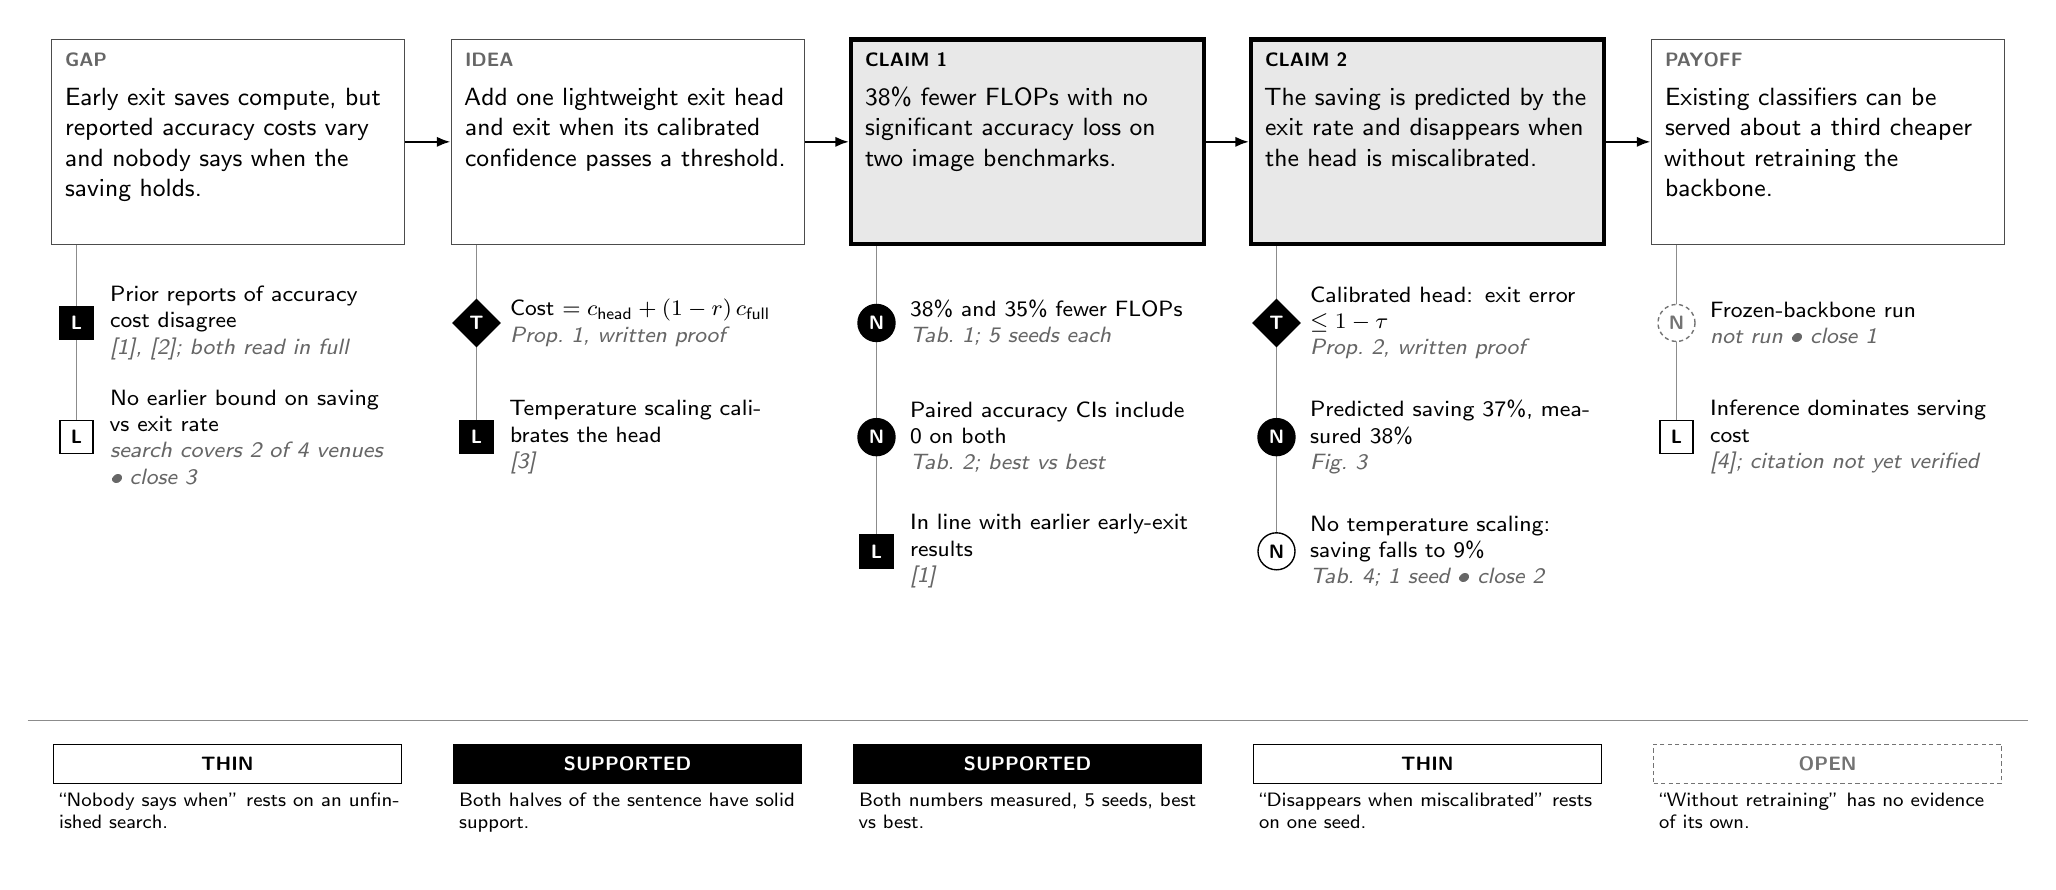
\begin{tikzpicture}[x=1cm,y=1cm]
\useasboundingbox (0,0) rectangle (25.4,{\vy-1.25});

% ---- spine: 4 to 6 beats, 1 or 2 of them \claim. Sentence <= 110 characters.
\beat{1}{GAP}{Early exit saves compute, but reported accuracy costs vary and nobody says when the saving holds.}
\beat{2}{IDEA}{Add one lightweight exit head and exit when its calibrated confidence passes a threshold.}
\claim{3}{CLAIM 1}{38\% fewer FLOPs with no significant accuracy loss on two image benchmarks.}
\claim{4}{CLAIM 2}{The saving is predicted by the exit rate and disappears when the head is miscalibrated.}
\beat{5}{PAYOFF}{Existing classifiers can be served about a third cheaper without retraining the backbone.}
\spinearrows

% ---- evidence: at most 4 rows per beat. Label <= 45 characters; pointer always given.
\stem{1}{2}
\ev{1}{1}{L}{solid}{Prior reports of accuracy cost disagree}{[1], [2]; both read in full}
\ev{1}{2}{L}{partial}{No earlier bound on saving vs exit rate}{search covers 2 of 4 venues \textbullet{} close 3}

\stem{2}{2}
\ev{2}{1}{T}{solid}{Cost $=c_{\text{head}}+(1-r)\,c_{\text{full}}$}{Prop.~1, written proof}
\ev{2}{2}{L}{solid}{Temperature scaling calibrates the head}{[3]}

\stem{3}{3}
\ev{3}{1}{N}{solid}{38\% and 35\% fewer FLOPs}{Tab.~1; 5 seeds each}
\ev{3}{2}{N}{solid}{Paired accuracy CIs include 0 on both}{Tab.~2; best vs best}
\ev{3}{3}{L}{solid}{In line with earlier early-exit results}{[1]}

\stem{4}{3}
\ev{4}{1}{T}{solid}{Calibrated head: exit error $\le 1-\tau$}{Prop.~2, written proof}
\ev{4}{2}{N}{solid}{Predicted saving 37\%, measured 38\%}{Fig.~3}
\ev{4}{3}{N}{partial}{No temperature scaling: saving falls to 9\%}{Tab.~4; 1 seed \textbullet{} close 2}

\stem{5}{2}
\ev{5}{1}{N}{missing}{Frozen-backbone run}{not run \textbullet{} close 1}
\ev{5}{2}{L}{partial}{Inference dominates serving cost}{[4]; citation not yet verified}

% ---- verdict per beat: supported / thin / open, plus the reason in <= 12 words.
\draw[black!45,line width=0.4pt] (0,\vy+0.55) -- (25.4,\vy+0.55);
\verdict{1}{thin}{``Nobody says when'' rests on an unfinished search.}
\verdict{2}{supported}{Both halves of the sentence have solid support.}
\verdict{3}{supported}{Both numbers measured, 5 seeds, best vs best.}
\verdict{4}{thin}{``Disappears when miscalibrated'' rests on one seed.}
\verdict{5}{open}{``Without retraining'' has no evidence of its own.}
\end{tikzpicture}

% ===================================================================== to close / scope
\rule{\linewidth}{0.4pt}\\[3pt]
\begin{minipage}[t]{0.60\linewidth}\small
\textbf{To close, in order of damage to the story} (at most 4)
\begin{enumerate}[label=\textbf{\arabic*.}]
\item Run the frozen-backbone experiment, or cut ``without retraining'' from the payoff.
\item Repeat the calibration ablation with 5 seeds.
\item Finish the prior-work search on the remaining two venues; read the closest paper in full.
\end{enumerate}
\end{minipage}\hfill
\begin{minipage}[t]{0.36\linewidth}\small
\textbf{Scope of the claims}\\
Two image benchmarks; one GPU type; batch size 1. ``No significant loss'' is not equivalence: no equivalence test was run.
\end{minipage}
\end{document}
